\documentclass[french]{article}
 
\usepackage[utf8]{inputenc}
\usepackage[T1]{fontenc}
\usepackage{babel}
\usepackage{graphicx}
\usepackage{amsmath}

\begin{document}
\section{Tension de surface}

la tension de surface est la l'énergie par unité de surface, c'est l'énergie nécessaire pour augmenter la surface d'une interface d'une unité.

\subsection{Mouillage}
Le mouillage est l'action de mouiller et mouiller consiste à  mettre en contact avec un liquide.
\begin{figure}[ht]
	\centering
	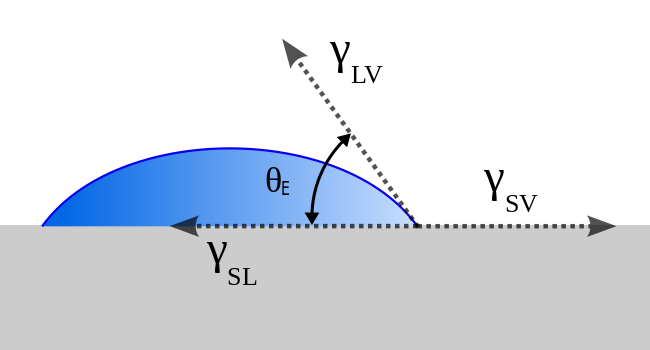
\includegraphics[scale = 0.3]{./image/Contact_angle2.png}
	\caption{Ligne triple}
\end{figure}

Nous nous intéressons en particulier au contact d'une goutte dont le support est une plaque plane. 


Le substrat est le nom donné au support (solide ou liquide) sur lequel la goutte de liquide repose.

Lorsqu'une d'eau est posée sur support solide il y a formation de 3 interfaces et donc de 3 tensions de surface.


C'est le paramètre d'étalement $S = \gamma_{SG} - \gamma_{SL} - \gamma_{LG}$ qui caractérise le mouillage lorsque la goutte est en équilibre.

En effet lorsque la goutte est en équilibre nous avons en projetant les tensions de surface sur l'horizontale, on a:

\begin{equation}
	\gamma_{SG}\ = \gamma_{SL} - \gamma_{LG}\cos\theta_{E}
\end{equation}
\begin{description}
\item[$S < 0$ :] Mouillage partiel
\item[$S > 0$ :] Mouillage total
\end{description}


Lorsque la goutte est en mouvement, l'angle dynamique   entre 2 liquides non miscibles ou entre un liquide et l'air ou en un liquide et une surface.

La tension de surface 

La capillarité étudie l'interface entre l'air et un liquide ou entre 2 liquides
non miscibles.

Le mouillage est l'action de mouiller et mouiller consiste à mettre en contact avec un liquide.

Nous nous intéressons en particulier au contact d'une goutte avec un support matériel.

C'est le paramètre d'étalement $S = \gamma_{SG} - \gamma_{SL} - \gamma_{LG}$ qui caractérise le mouillage lorsque la goutte est en équilibre sur un support matériel.

\begin{description}
\item[$S < 0$ :] Mouillage partiel
\item[$S > 0$ :] Mouillage total
\end{description}

Lorsque la que est en équilire nous avons:

\[\gamma_{SG}\ = \gamma_{SL} - \gamma_{LG}\cos\theta_{E} \]

\begin{figure}[ht]
	\centering
	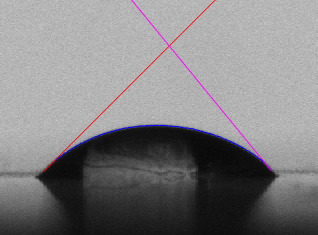
\includegraphics[scale = 0.6]{./image/crop_tvitesse=28_volume=003.png}
	\caption{Goutte d'eau de volume $0.03$ml avec $\theta_{a} = 45^{o}$ et $\theta_{r} = 50.17^{o}$}
\end{figure}

\begin{figure}[ht]
	\centering
	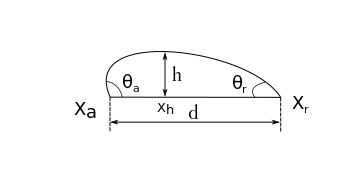
\includegraphics[scale = 0.6]{./image/rrgou.png}
	\caption{Goutte d'eau de volume $0.03$ml}
\end{figure}
\end{document}
